%!TEX program = xelatex
% 完整编译: xelatex -> bibtex -> xelatex -> xelatex
\documentclass[lang=cn,a4paper,cite=authoryear]{elegantpaper}
\songti

\title{\zihao{1}哈尔滨工业大学计算机科学与技术学院 \par 实验报告}
\date{}
% 本文档命令
\usepackage{array}
\usepackage{enumitem}
\usepackage{graphicx}
\usepackage{minted}
\usepackage{subfigure}
\newcommand{\ccr}[1]{\makecell{{\color{#1}\rule{1cm}{1cm}}}}

\begin{document}

\maketitle
\thispagestyle{empty}
\begin{center}
	\zihao{3}
   	{ 课程名称:  机器学习}\\[.5cm]
    { 课程类型:   选修}\\[.5cm]
    { 实验题目:  PCA模型实验}\\[.5cm]
	{ 学 号:  1190202110}\\[.5cm]
	{ 姓 名: 田雪洋}\\[.5cm]
    { \date{\zhtoday}}\\[.50cm]
\end{center}


\newpage
\zihao{4}
\section*{\zihao{2}{一、实验目的}}
目标:实现一个PCA模型,能够对给定数据进行降维(即找到其中的主成分)

\section*{\zihao{2}{二、实验要求及实验环境}}
\subsection*{\zihao{-2}{1.实验要求}}
目标:实现一个PCA模型,能够对给定数据进行降维(即找到其中的主成分)
\par 测试:(1)首先人工生成一些数据(如三维数据),让它们主要分布在低维空间中,如首先让某个维度的方差远小于其它唯独,然后对这些数据旋转。生成这些数据后,用你的PCA方法进行主成分提取。
\par (2)找一个人脸数据(小点样本量),用你实现PCA方法对该数据降维,找出一些主成分,然后用这些主成分对每一副人脸图像进行重建,比较一些它们与原图像有多大差别(用信噪比衡量)。


\subsection*{\zihao{-2}{2.实验环境}}
Windows10; python3.8.6;Pycharm 
\section*{\zihao{2}{三、设计思想(本程序中的用到的主要算法及数据结构)}}
PCA(Principal Component Analysis),即主成分分析方法,是一种使用最广泛的数据降维算法。其基本原理是利用正交变换把由线性相关变量表示的观测数据转换为少数几个由线性无关变量表示的数据,这些线性无关变量称为主成分,且主成分的个数通常小于原始变量的个数。下面从两个不同的角度实现PCA
\subsection*{\zihao{-2}{1.最大投影方差}}
对于一组观测数据$x=\left( \boldsymbol{x}_1,\boldsymbol{x}_2,\cdots ,\boldsymbol{x}_{\boldsymbol{n}} \right)$,$x_i$是m维随机变量,我们首先对$x_i$进行中心化,中心化可以给后面的计算带来极大的便利,因为中心化之后的常规线性变换就是绕原点的旋转变化,也就是坐标变换。
然后, 为了方便推导,我们定义:
样本均值:
\begin{equation}
	\bar{x}=\frac{1}{n} \sum_{i}^{n} x_{i}
\end{equation}
样本投影均值:
\begin{equation}
	\mu=\frac{1}{n} \sum_{i}^{n} w^{T} x_{i}
\end{equation}
样本的协方差矩阵:
\begin{equation}
	\operatorname{cov}(X)=\Sigma=\frac{1}{n} \sum_{i}^{n}\left(x_{i}-\bar{x}\right)\left(x_{i}-\bar{x}\right)^{T}
\end{equation}
样本在$w$上的投影后的方差为:
\begin{equation}
	\begin{aligned}
		\sigma^{2} &=\frac{1}{n} \sum_{i}^{n}\left(w^{T} x_{i}-\mu\right)^{2} \\
		&=\frac{1}{n} \sum_{i}^{n}\left(w^{T} x_{i}-\frac{1}{n} \sum_{i}^{n} w^{T} x_{i}\right)^{2} \\
		&=\frac{1}{n} \sum_{i}^{n}\left(w^{T} x_{i}-w^{T}\left(\frac{1}{n} \sum_{i}^{n} x_{i}\right)\right)^{2} \\
		&=\frac{1}{n} \sum_{i}^{n}\left(w^{T}\left(x_{i}-\bar{x}\right)\right)^{2} \\
		&=\frac{1}{n} \sum_{i}^{n}\left(w^{T}\left(x_{i}-\bar{x}\right)\right)\left(w^{T}\left(x_{i}-\bar{x}\right)\right)^{T} \\
		&=\frac{1}{n} \sum_{i}^{n} w^{T}\left(x_{i}-\bar{x}\right)\left(x_{i}-\bar{x}\right)^{T} w \\
		&=w^{T}\left[\frac{1}{n} \sum_{i}^{n}\left(x_{i}-\bar{x}\right)\left(x_{i}-\bar{x}\right)^{T}\right] w \\
		&=w^{T} \Sigma w
	\end{aligned}
\end{equation}
为了在降维的同时,尽可能保留原样本的信息,因此,我们需要让样本点在投影的超平面内尽可能的散开,这里使用方差衡量投影后的离散程度。这就是最大投影方差的主要思想。而要求方差最大的投影面,即,
\begin{equation}
	\hat{w}=\arg \max _{w} w^{T} \Sigma w
\end{equation}
而另一方面,为了表示投影方便,我们规定$w$为单位向量,即$ww^T=1$。综上,根据拉格朗日乘数法,得到优化的目标函数为:
\begin{equation}
	L(w, \lambda)=w^{T} \Sigma \mathbf{w}+\lambda\left(1-w^{T} w\right)
\end{equation}
对目标函数求导,得到
\begin{equation}
	\frac{\partial L(w, \lambda)}{\partial w}=2 \Sigma w-2 \lambda w
\end{equation}
令该式为0,求得:
\begin{equation}
	\Sigma w=\lambda w
\end{equation}
由特征值和特征向量的定义可以看出,$\lambda$是$\Sigma$的特征值,$w$是$\Sigma$的特征向量。
\par 对于(4)式,我们将(8)式中的结果代入得到:
\begin{equation}
	\sigma^{2} =\lambda
\end{equation}
所以,我们仅需要求出前k大的特征值,即可求出前k大的特征向量,即投影面。
\par 此外由于我们对数据进行了中心化处理,所以(1)式的均值实际上就是0,则协方差矩阵可以写成:
\begin{equation}
	\operatorname{cov}(X)=\Sigma=\frac{1}{n} X X^{T}
\end{equation}
(10)式得到的协方差矩阵为对称矩阵,所以我们可以得到如下特征分解:
\begin{equation}
	\Sigma=G \Lambda G^{T}
\end{equation}
其中G是$\Sigma$的特征向量组成的矩阵,$ \Lambda$是相对应的特征值组成的对角矩阵,我们仅需要使该对角矩阵中的元素取前k大的特征值即可,求出最终的答案。
具体算法过程如下:
\begin{enumerate}[(1)]
\item 设有n个m维的随机变量$x=\left( \boldsymbol{x}_1,\boldsymbol{x}_2,\cdots ,\boldsymbol{x}_{\boldsymbol{n}} \right)$
\item 将x的每一行进行中心化,即减去这一行的均值,是均值为0;
\item 求出协方差矩阵$\operatorname{cov}(X)=\Sigma=\frac{1}{n} X X^{T}$;
\item 求出协方差矩阵对应的特征值和特征向量;
\item 将特征向量按对应特征值大小从上到下按列排列成矩阵,取前k列组成矩阵w;
\item 则$y=w^{T}x$即为降维到 k 维后的数据。
\end{enumerate}
\subsection*{\zihao{-2}{2.最小投影距离}}
除了最大投影方差,PCA也可以从最小投影距离的角度进行推导。显然,对于中心化后的数据样本点,坐标原点的距离不变,而投影面的方差最大,也就等价于这些样本点到投影面的距离最小。所以,下面从最小投影距离的角度推导PCA。
\par 对于中心化后的数据$x=\left(x^{(1)}, x^{(2)}, \ldots, x^{(n)}\right)$,我们定义$z^{(i)}=\left(z_{1}^{(i)}, z_{2}^{(i)}, \ldots, z_{k}^{(i)}\right)^{T}$为经过投影变换后新坐标系中$x^{(i)}$的k维坐标。其中,$z_{j}^{(i)}=w_{j}^{T} x^{(i)}$
\par 那么,当我们采用$z_{j}$去恢复$x^{(i)}$时会得到恢复数据$\bar{x}^{(i)}$,最小投影距离也就是求得:
\begin{equation}
   \operatorname{argmin} \sum_{i=1}^{n}\left\|\bar{x}^{(i)}-x^{(i)}\right\|_{2}^{2}
\end{equation}
对该式化简得到:
\begin{equation}
	\begin{aligned}
		\sum_{i=1}^{n}\left\|\bar{x}^{(i)}-x^{(i)}\right\|_{2}^{2} &=\sum_{i=1}^{m}\left\|W z^{(i)}-x^{(i)}\right\|_{2}^{2} \\
		&=\sum_{i=1}^{m}\left(W z^{(i)}\right)^{T} W z^{(i)}-2 \sum_{i=1}^{m}\left(W z^{(i)}\right)^{T} x^{(i)}+\sum_{i=1}^{m} x^{(i) T} x^{(i)} \\
		&=\sum_{i=1}^{m}\left(z^{(i) T}\right) z^{(i)}-2 \sum_{i=1}^{m}\left(z^{(i) T}\right) W^{T} x^{(i)}+\sum_{i=1}^{m} x^{(i) T} x^{(i)} \\
		&=\sum_{i=1}^{m}\left(z^{(i) T}\right) z^{(i)}-2 \sum_{i=1}^{m}\left(z^{(i) T}\right) z^{(i)}+\sum_{i=1}^{m} x^{(i) T} x^{(i)} \\
		&=-\sum_{i=1}^{m}\left(z^{(i) T}\right) z^{(i)}+\sum_{i=1}^{m} x^{(i) T} x^{(i)} \\
		&\left.=-\operatorname{tr}\left(W^{T} \sum_{i=1}^{m}\left(x^{(i) T}\right) x^{(i)}\right) W\right)+\sum_{i=1}^{m} x^{(i) T} x^{(i)} \\
		&=-\operatorname{tr}\left(W^{T} X X^{T} W\right)+\Sigma
	\end{aligned}
\end{equation}
由于协方差矩阵$\Sigma$是不变的,所以最小化(13)式等于最小化:
\begin{equation}
	\begin{aligned}
		&\operatorname{argmax} \quad \operatorname{tr}\left(W^{T} X X^{T} W\right) \\
		&\text { s.t. } \quad W^{T} W=I
	\end{aligned}
\end{equation}
这个结果与前面的最大投影误差法得到的结果相同。
\section*{\zihao{2}{四、实验结果与分析}}
\subsection*{\zihao{-2}{1.生成数据}}
为了方便进行数据可视化,在这里只使用了2维数据和3维数据的在PCA前后的对比实验。
\subsubsection*{\zihao{3}{(1).二维降到一维}}
在这里,生成$\mu=[-2,2]$和$\Sigma=[[1,0],[0,0.01]]$的二维高斯分布,可以看到在第二维的方差远小于第一维的方差,因此,第二维包含了更多的信息,进行PCA降维的结果如下:
\begin{center}
	\begin{figure}[H]
		\centering
		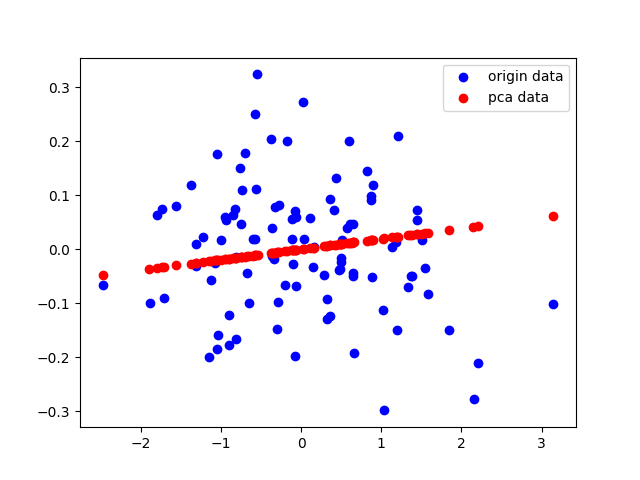
\includegraphics[scale=0.6]{test01}
	\end{figure}
\end{center}
可以看到PCA降维的结果基本上分布在与第一维平行的直线上,且第一维的方差极小,第二维的方差较大,符合预期。
\subsubsection*{\zihao{3}{(1).三维降到二维}}
在这里,生成$\mu=[1, 2, 3]$和$\Sigma=[[0.01, 0, 0], [0, 1, 0], [0, 0, 1]]$的三维高斯分布,可以看到在第一维的方差远小于第二维和第三维的方差,因此,第二维和第三维包含了更多的信息,进行PCA降维的结果如下:
\begin{figure}[H]
	\centering  %图片全局居中
	\subfigure[视角1]{
		\label{Fig.sub.1}
		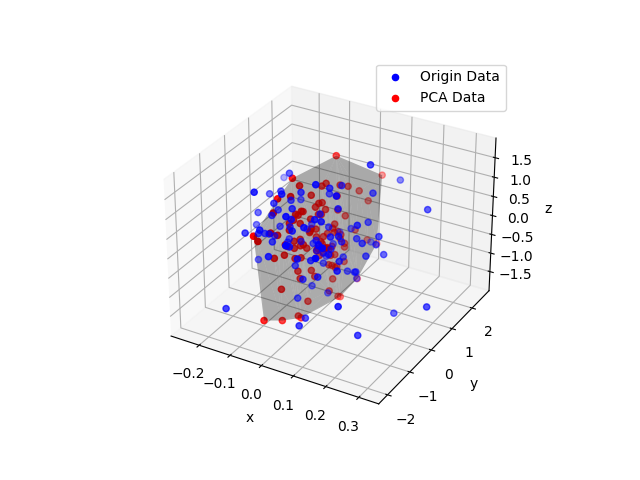
\includegraphics[width=0.48\textwidth]{test02}}
	\subfigure[视角2]{
		\label{Fig.sub.2}
		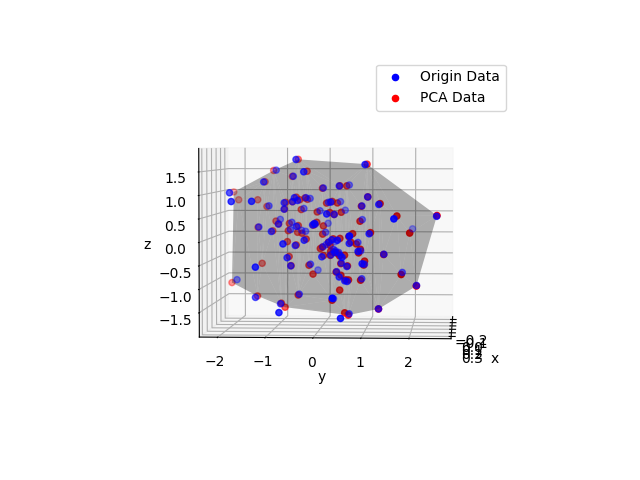
\includegraphics[width=0.48\textwidth]{test04}}
	
		\subfigure[视角3]{
		\label{Fig.sub.3}
		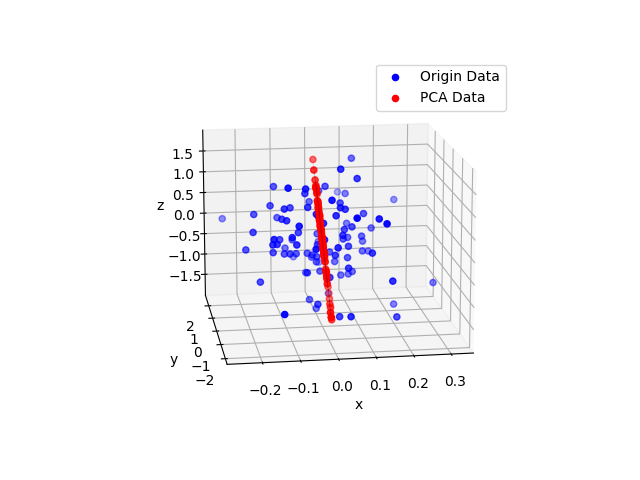
\includegraphics[width=0.48\textwidth]{test03}}
			\subfigure[视角4]{
		\label{Fig.sub.4}
		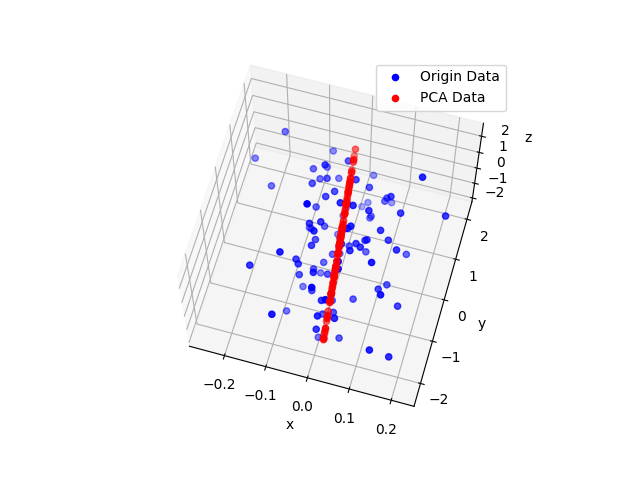
\includegraphics[width=0.48\textwidth]{test05}}
	\caption{不同视角下的PCA结果}
	\label{Fig.main}
\end{figure}
可以看到PCA降维的结果基本上分布在第二维第三维组成的平面,符合预期。
\subsection*{\zihao{-2}{2.人脸数据测试}}
图像的信噪比和图像的清晰度一样,都是衡量图像质量高低的重要指标。图像的信噪比是指视频信号的大小与噪波信号大小的比值,其公式为:
\begin{equation}
	\begin{aligned}
		&M S E=\frac{1}{M N} \sum_{i=0}^{M-1} \sum_{j=0}^{N-1}\|I(i, j)-K(i, j)\|^{2} \\
		&P S N R=10 \cdot \log _{10}\left(\frac{M A X_{I}^{2}}{M S E}\right)=20 \cdot \log _{10}\left(\frac{M A X_{I}}{\sqrt{M S E}}\right)
	\end{aligned}
\end{equation}
下面分别使用一男一女两组人脸图片利用PCA进行降维处理,并计算信噪比:
\begin{figure}[H]
	\centering  %图片全局居中
	\subfigure[原图片($227\times305$)]{
		\label{Fig.sub.1}
		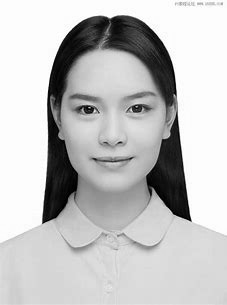
\includegraphics[scale=0.5]{gface01}}
	\subfigure[$k=100,PSNR=44.985$]{
		\label{Fig.sub.2}
		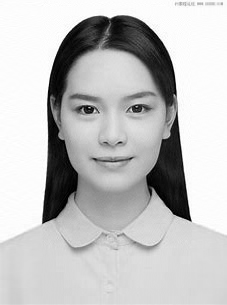
\includegraphics[scale=0.5]{gface02}}
	\subfigure[$k=50,PSNR=34.780$]{
		\label{Fig.sub.3}
		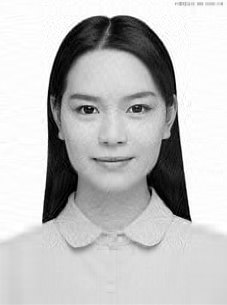
\includegraphics[scale=0.5]{gface03}}
	
	\subfigure[$k=10,PSNR=24.571$]{
		\label{Fig.sub.4}
		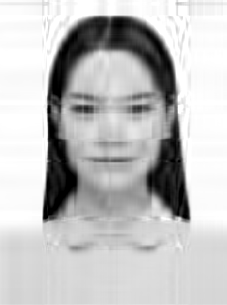
\includegraphics[scale=0.5]{gface04}}
	\subfigure[$k=5,PSNR=21.515$]{
		\label{Fig.sub.5}
		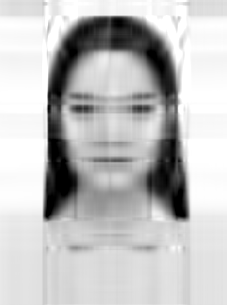
\includegraphics[scale=0.5]{gface05}}
	\subfigure[$k=1,PSNR=14.716$]{
		\label{Fig.sub.7}
		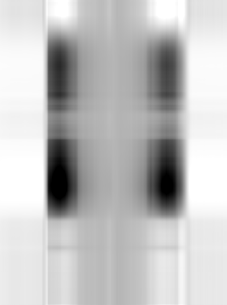
\includegraphics[scale=0.5]{gface07}}
	\caption{女性人脸图像降维结果}
	\label{Fig.main}
\end{figure}
\begin{figure}[H]
	\centering  %图片全局居中
	\subfigure[原图片($238\times238$)]{
		\label{Fig.sub.1}
		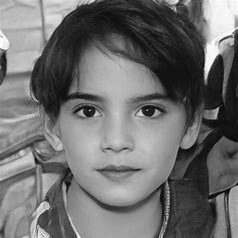
\includegraphics[scale=0.5]{bface01}}
	\subfigure[$k=100,PSNR=41.808$]{
		\label{Fig.sub.2}
		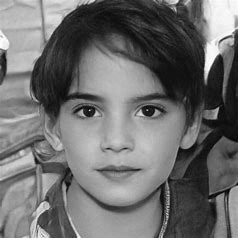
\includegraphics[scale=0.5]{bface02}}
	\subfigure[$k=50,PSNR=33.206$]{
		\label{Fig.sub.3}
		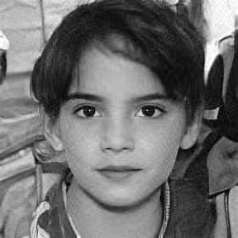
\includegraphics[scale=0.5]{bface03}}
	
	\subfigure[$k=10,PSNR=23.646$]{
		\label{Fig.sub.4}
		\includegraphics[scale=0.5]{bface04 }}
	\subfigure[$k=5,PSNR=20.896$]{
		\label{Fig.sub.5}
		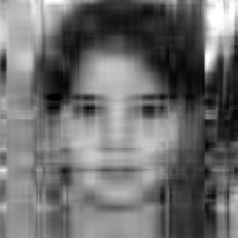
\includegraphics[scale=0.5]{bface05}}
	\subfigure[$k=1,PSNR=16.466$]{
		\label{Fig.sub.7}
		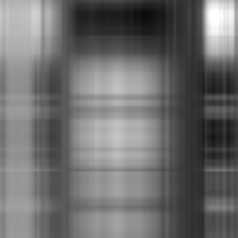
\includegraphics[scale=0.5]{bface07}}
	\caption{男性人脸图像降维结果}
	\label{Fig.main}
\end{figure}




\section*{\zihao{2}{五、结论}}
\begin{itemize}
\item PCA算法中舍弃了较小的几个特征值对应的特征向量,有效提高了样本的采样密度;而且由于特征值对较小的几个特征向量往往与噪声有关,因此,PCA同时也起到了降噪的效果
\item PCA不仅将数据压缩到低维,并且将降维之后的各维特征相互独立。

\end{itemize}
\section*{\zihao{2}{六、参考文献}}
\begin{enumerate}[(1)]
\item  周志华 著. 机器学习, 北京: 清华大学出版社, 2016.1
\item  李航 著. 统计学习方法,北京:清华大学出版社,2020.6
\end{enumerate}
\section*{\zihao{2}{七、附录:源代码(带注释)}}
源代码见相关文件
\begin{enumerate}[(1)]
	\item  bfacetest.py:测试男性人脸图片使用PCA降维效果
	\item  gfacetest.py:测试女性人脸图片使用PCA降维效果
	\item  data.py:数据预处理及PCA算法实现
	\item  test2D.py:利用PCA将二维数据降维成一维数据的测试
	\item  test3D.py:利用PCA将三维数据降维成二维数据的测试
\end{enumerate}
\end{document}